\documentclass{beamer}
\usepackage{appendixnumberbeamer}

\mode<presentation>{\usetheme[subsectionpage=progressbar,block=fill,numbering=none]{metropolis}}

\usepackage[english]{babel} 
\usepackage[utf8]{inputenc}

\usepackage{standalone}
\usetikzlibrary{calc,arrows.meta,positioning}
\usepackage{tikz-3dplot}
\usepackage{graphicx} % Allows including images
\usepackage{tikz}
\usepackage{pgfplots}
\pgfplotsset{compat=1.13}
\usepackage{pgfplotstable}
\usepackage{caption}
\usepackage{booktabs} % Allows the use of \toprule, \midrule and \bottomrule in tables
\usepackage{multicol} 

% Math packages
\usepackage{amsmath}
\usepackage{mathtools}
\usepackage{amssymb}
\usepackage{mathpartir}

% Coloured boxes
\usepackage{tcolorbox}
\colorlet{alert}{mLightBrown}
\newtcolorbox{alertbox}
{standard jigsaw, opacityback=0,colframe=alert}
\newtcolorbox{tbox}
{standard jigsaw, opacityback=0,opacityframe=0}

% Custom commands
\DeclarePairedDelimiter\ceil{\lceil}{\rceil}
\DeclarePairedDelimiter\floor{\lfloor}{\rfloor}
\DeclareMathOperator*{\argmin}{arg\,min}
\DeclareMathOperator*{\argmax}{arg\,max}
\newcommand{\mx}{\mathcal{X}}
\newcommand{\inp}{\mathcal{I}}
\newcommand{\costs}{c}
\newcommand{\opcosts}{c_{op}}
\newcommand{\swcosts}{c_{sw}}
\newcommand{\aswcosts}{\widehat{c}_{sw}}
\newcommand{\beps}{\boldsymbol\varepsilon}
\newcommand{\fromto}[2]{\{#1,\dotsc,#2\}}
\newcommand{\dotcup}{\mathbin{\mathaccent\cdot\cup}}

\title{Algorithms for Dynamic Right-Sizing in\\Data Centers} % The short title appears at the bottom of every slide, the full title is only on the title page

\author{Kevin Kappelmann} % Your name
\institute[TUM]{Technical University of Munich}
\date{\today} % Date, can be changed to a custom date

\begin{document}
\maketitle

%------------------------------------------------
\section{Model and Problem Formulation}
%------------------------------------------------
\begin{frame}{Model Description}
Input:
\begin{itemize}[<+->]
  \item $m\in\mathbb{N}$\dotso Number of homogeneous servers 
  \item $\beta\in\mathbb{R}_{\ge 0}$\dotso Switching costs of a server
  \item $f:[0,1]\rightarrow\mathbb{R}$\dotso Convex operating cost function of a server
  \item $T\in\mathbb{N}$\dotso Number of time slots
  \item $\lambda_1,\dotsc,\lambda_{T}\in[0,m]$\dotso Arrival rates (workloads)
\end{itemize}
\pause[\thebeamerpauses]
Notation:
\begin{itemize}
	\item $x_1,\dotsc,x_{T}\in\fromto{0}{m}$\dotso Numbers of active servers
\end{itemize}
\end{frame}
%------------------------------------------------
\begin{frame}{Problem Statement}
Operating costs for one time step $t$
\begin{equation*}
	\opcosts(x_t,\lambda_t)\coloneqq\begin{cases}
	  \pause\infty, & \text{if $\lambda_t>x_t$}\hspace{16mm}\text{//too few servers}\\
          \pause 0, & \text{if $x_t=\lambda_t=0$\hspace{9mm}\text{//no active servers}}\\
	  \pause x_tf(\lambda_t/x_t), & \text{otherwise}\hspace{16mm}\text{//even distribution}
	  \end{cases}
\end{equation*}
\pause
\begin{alertbox}
\centering \textbf{Goal: Minimize total costs}
\begin{align*}
	\text{minimize}\quad \sum\limits_{t=1}^{T}\Bigl(\underbrace{\opcosts(x_t,\lambda_t)+\beta\max\{0,x_t-x_{t-1}\}}_{\costs(x_{t-1},x_t,\lambda_t)}\Bigr)
\end{align*}
\end{alertbox}
\end{frame}
%------------------------------------------------
\section{Optimal Offline Algorithm}
%------------------------------------------------
\begin{frame}{Pseudo-Linear-Time Algorithm}
\centerline{Fundamental idea: reduce problem to shortest path problem}
\pause
\begin{figure}
	\includestandalone[width=\textwidth]{../thesis/figures/graph_pseudo_lin}
\end{figure}
\pause \centering{Time complexity: $\Theta(Tm)$}

\pause\ldots only $\log_2(m)$ bits required to encode $m$.
\end{frame}
%------------------------------------------------
\section{Offline Approximation Algorithm}
%------------------------------------------------
\begin{frame}{2-Optimal Linear-Time Algorithm}
\centerline{Use logarithmic steps to reduce number of nodes}
\pause
\begin{figure}
	\includestandalone[width=\textwidth]{../thesis/figures/graph_lin_approx_2}
\end{figure}
\centering where $b\coloneqq\floor{\log_2(m)}$
\end{frame}
%------------------------------------------------
\begin{frame}{Approximative Scheduling}
Shortest Path in graph corresponds to 2-optimal schedule.

\pause Time complexity: $\Theta\bigl(T\log_2(m)\bigr)$
\vspace{\baselineskip}
\pause\begin{alertbox} 
\centering Approach can be generalized to allow for arbitrary precisions\\with time complexity $\Theta\bigl(T\log_{1+\beps}(m)\bigr)=\Theta\left(T\,\frac{\log(m)}{\log(1+\beps)}\right)$
\end{alertbox}
\end{frame}
%------------------------------------------------
\section{Summary and Prospects}
%------------------------------------------------
\begin{frame}{Summary}
We reduced the scheduling problem to the shortest path problem of acyclic graphs.

\pause
\begin{alertbox}
\centering Optimal Offline Algorithm with runtime $\Theta(Tm)$
\end{alertbox}
\pause
\begin{alertbox}
\centering $(1+\beps)$-Optimal Offline Algorithm with runtime $\Theta\left(T\,\frac{\log(m)}{\log(1+\beps)}\right)$
\end{alertbox}
\end{frame}
%------------------------------------------------
\begin{frame}{Prospects}
Can our approach be modified to\dotso
\pause
\begin{itemize}[<+->]
	\item deal with more than one homogeneous server collection?
	\item deal with multiple sleep states?
	\item work as an online algorithm?
\end{itemize}
\pause[\thebeamerpauses]
Open question: Is there a polynomial optimal algorithm or is it an $\textbf{NP}$ problem?
\end{frame}
%------------------------------------------------
\begin{frame}[standout]
Thanks for your attention!

Any questions?
\end{frame}
%----------------------------------------------------------------------------------------
%------------------------------------------------
\begin{frame}{Data Centers' Costs}
\centering{\Large Fast-growing demand for data collection, processing, and storage}

\vspace{0.5\baselineskip}
\visible<2>{\centering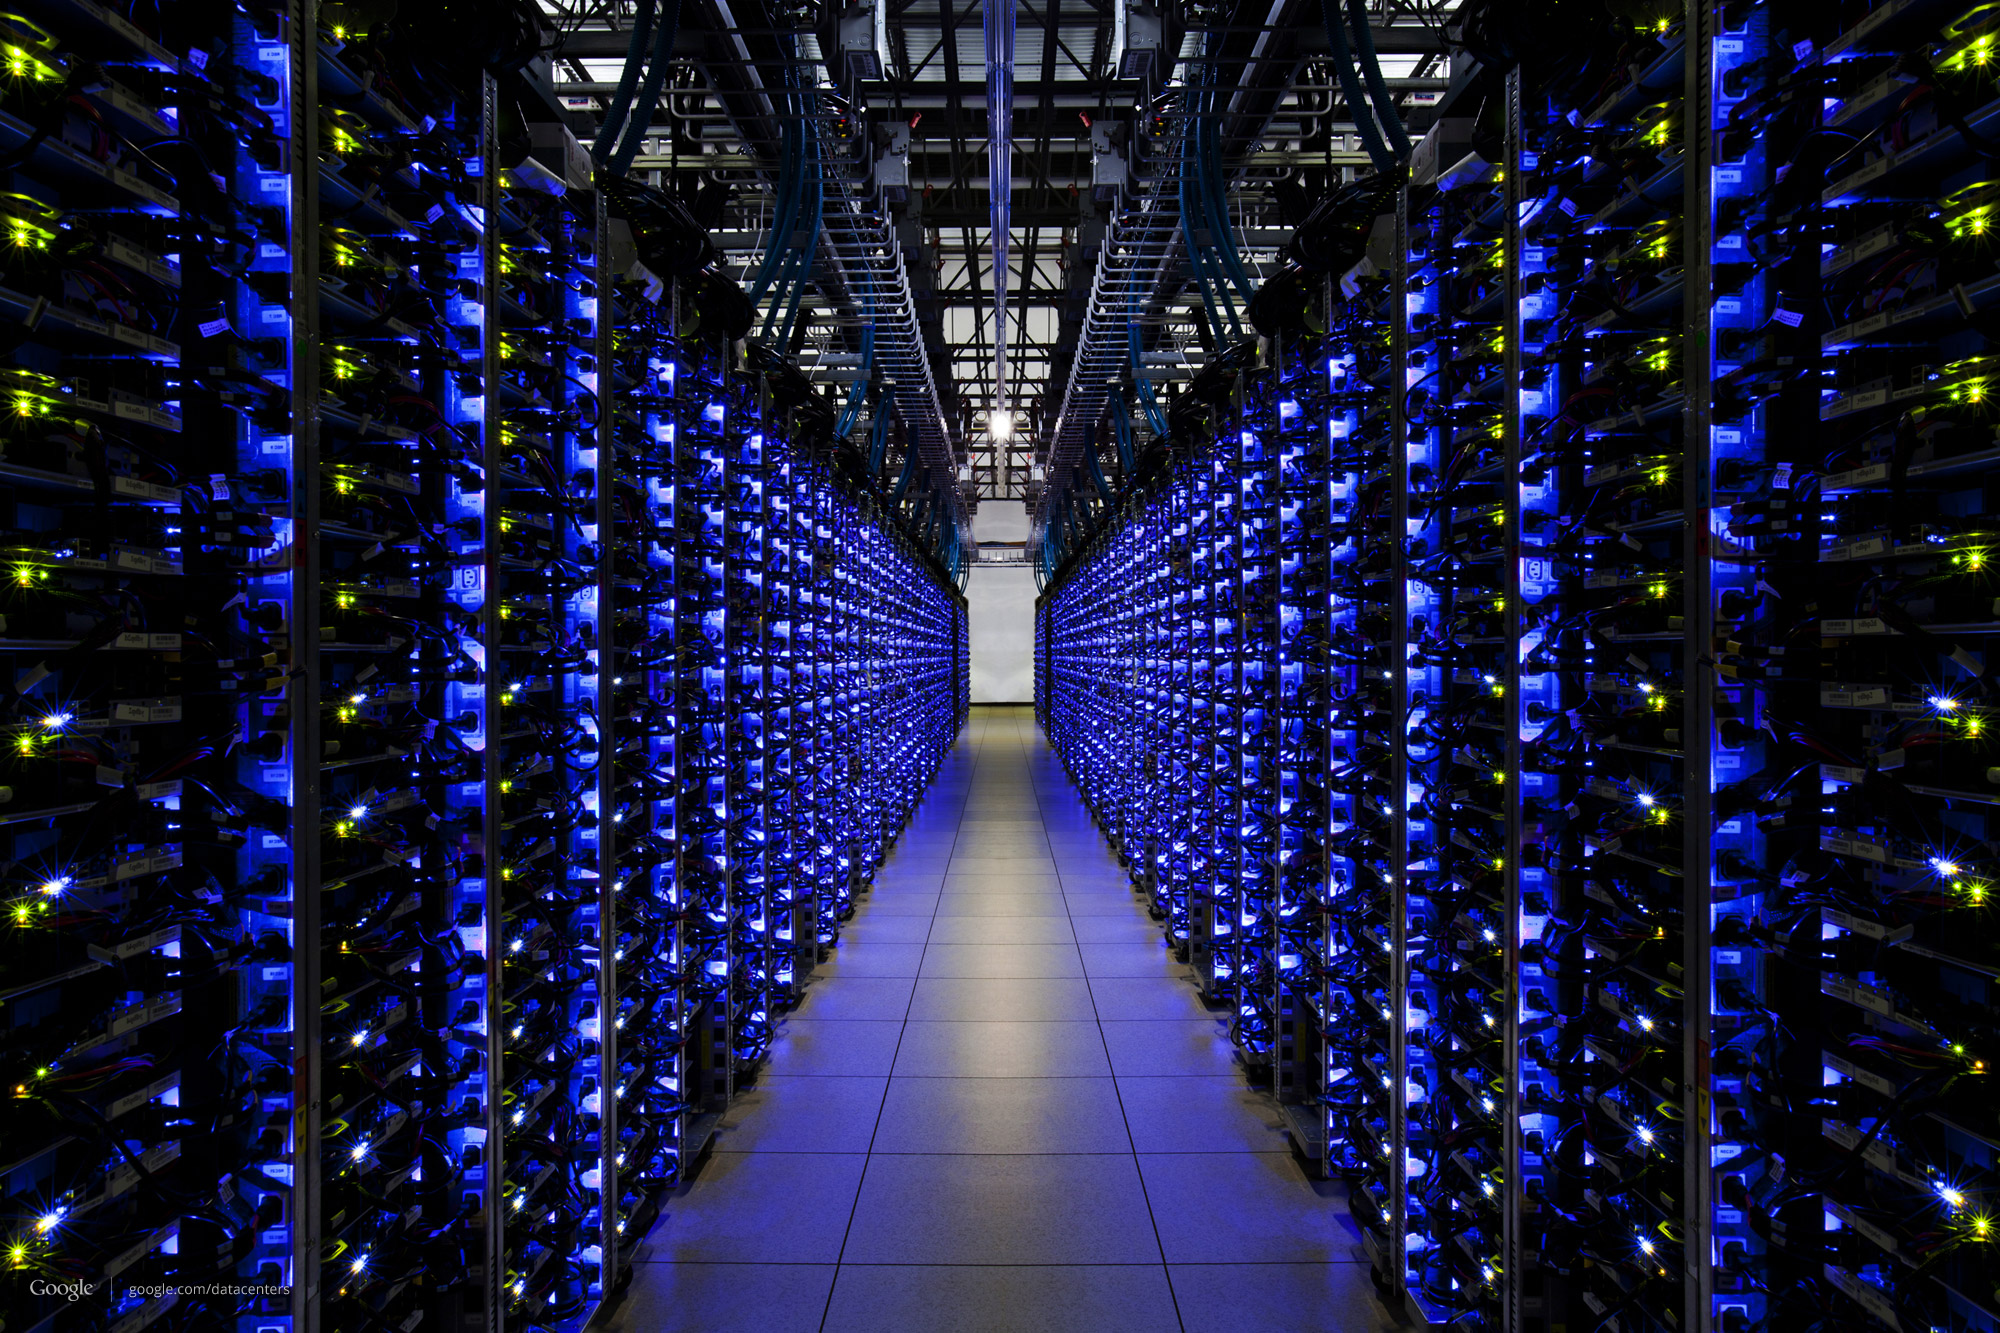
\includegraphics[height=0.5\textheight]{img/data_center.jpg}}
\end{frame}
%------------------------------------------------
\begin{frame}{Data Centers' Costs}
\centering{\Large Fast-growing demand for data collection, processing, and storage}

\vspace{0.5\baselineskip}
\centering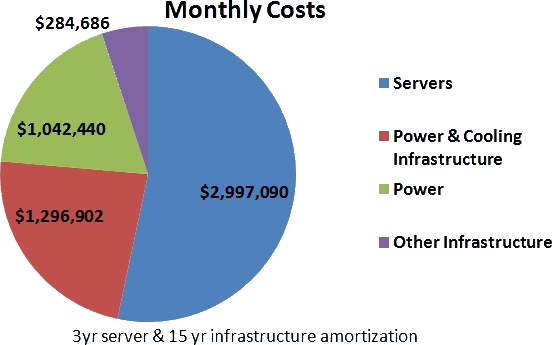
\includegraphics[height=0.5\textheight]{img/data_center_costs.jpg}
\end{frame}
%------------------------------------------------
\begin{frame}{Proof Idea}
\centering Take a schedule and transform periods between two powers of 2

\pause\begin{figure}
	\includestandalone[width=0.85\textwidth]{figures/schedule_behavior}
\end{figure}
\end{frame}
%------------------------------------------------
\begin{frame}{$(1+\beps)$-Optimal Offline Algorithm}
\begin{figure}
	\includestandalone[width=\textwidth]{../thesis/figures/graph_lin_approx_y}
\end{figure}
\centering where $y\coloneqq1+\beps$
\end{frame}
%------------------------------------------------
\begin{frame}[allowframebreaks]{Image Sources}
\begin{itemize}
\item Data center: \url{datacentervoice.com/wp-content/uploads/2015/12/data-center.jpg}
\item Data center costs: \url{perspectives.mvdirona.com/2008/11/cost-of-power-in-large-scale-data-centers/}
\end{itemize}
\end{frame}

\end{document} 
